\section{Resoconto delle attivita' di verifica\textsubscript{G}}

\subsection{Documentazione}

\subsubsection{Indice di Gulpease}

\begin{table}[H]
	\centering
	\setlength\extrarowheight{5pt}
	\rowcolors{2}{gray!10}{gray!40}
	\renewcommand\tabularxcolumn[1]{>{\Centering}m{#1}}
	\begin{tabularx}{\textwidth}{| c | X |} 
		\hline
		\rowcolor{white}
		\textbf{Documento} & \textbf{Valore}\\
		\hline
		\textit{Analisi\_dei\_Requisiti v 1.0.0} & 90 \\
		\hline
		\textit{Norme\_di\_Progetto v 1.0.0} & 75\\
		\hline
		\textit{Piano\_di\_Progetto v 1.0.0} & 68\\
		\hline
		\textit{Piano\_di\_Qualifica v 1.0.0} & 84\\
		\hline
		\textit{Glossario v 1.0.0} & 69\\
		\hline
		\rowcolor{white}
		\caption{Indice di Gulpease}
	\end{tabularx}
\end{table}
\begin{figure}[H]
	\centering
	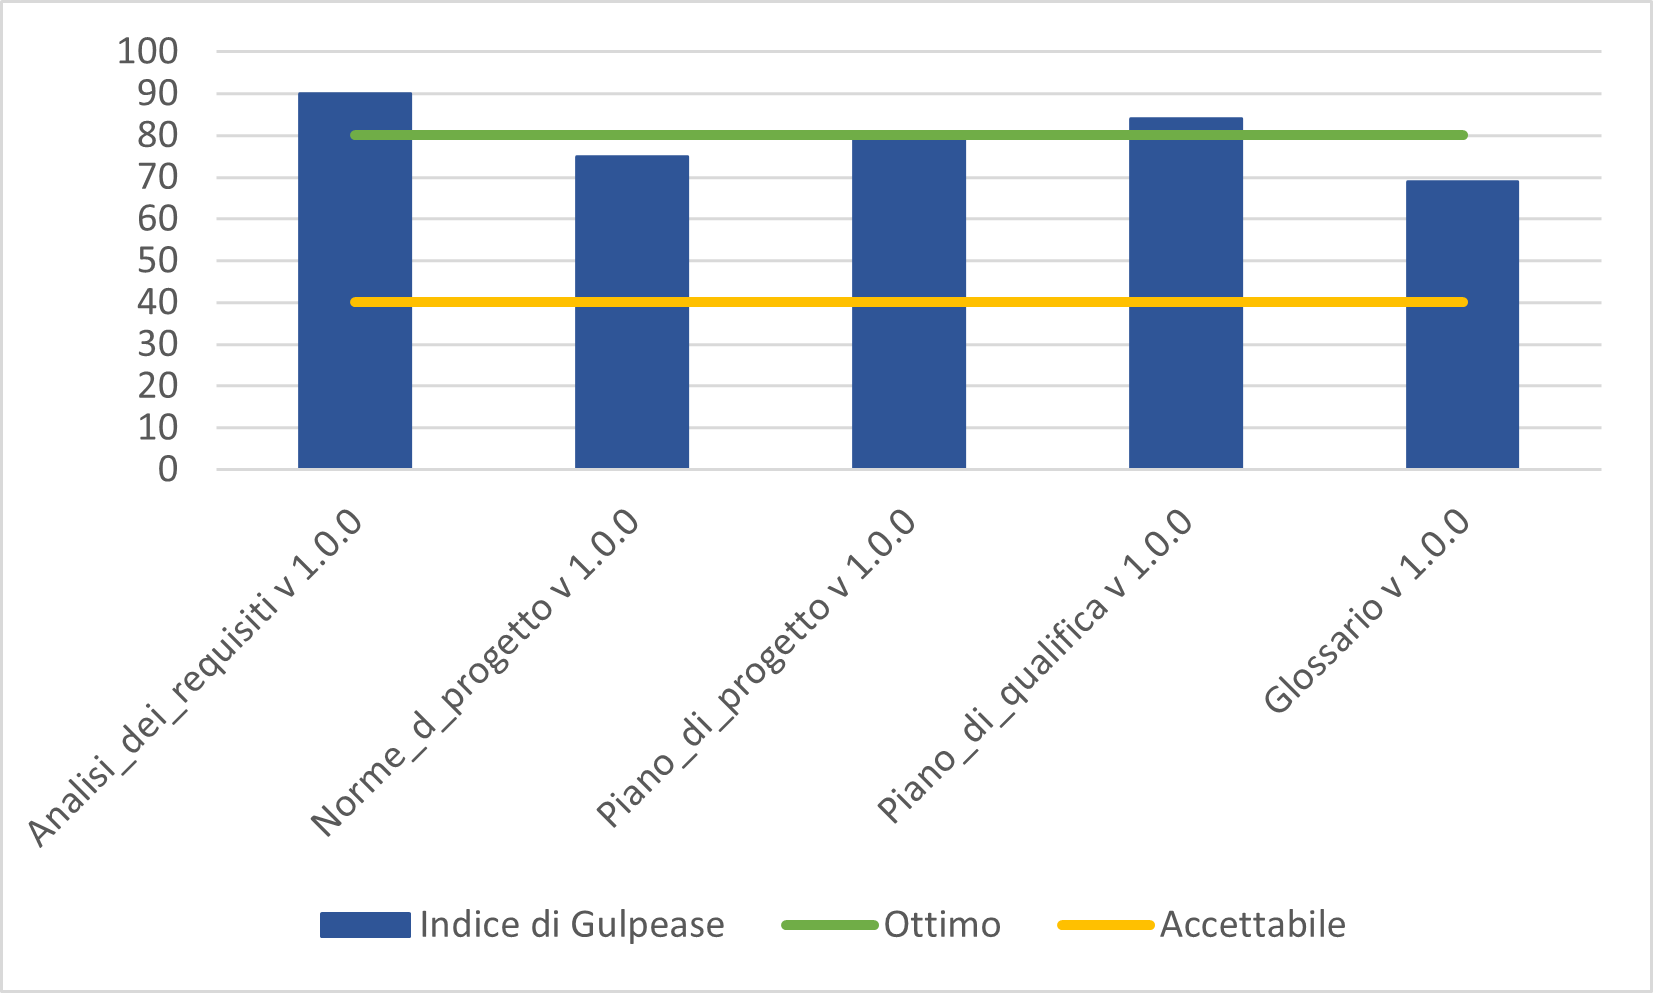
\includegraphics[scale=1.1]{img/Gulpease.png}
	\caption{Grafico che mostra l'indice di Gulpease per i vari documenti redatti}
\end{figure}
\paragraph{Analisi retrospettiva sui risultati}\mbox{}\\
I risultati ottenuti dai documenti sono soddisfacenti e superano la soglia che il gruppo ha definito accettabile. Tutti i documenti rilasciati hanno quindi un indice di leggibilità più che accettabile, alcuni superando anche l'ottimo definito. Non è stato calcolato l'indice sui vari verbali redatti, dato è stato utilizzato il template fornito dal servizio confluence di JIRA\textsubscript{G} per scriverli.
